\documentclass[12pt]{book} 

\usepackage{amsmath}
\usepackage{graphicx}
\usepackage{import}
\usepackage{amsfonts}
\usepackage{booktabs}

\setlength{\parindent}{0em}  % sets auto indent at new paragraph to none

\newcommand{\incfig}[1]{%
    \import{./figures/}{#1.pdf_tex}
}

\title{\coursetitle\linebreak\lecturename}
\author{\\Cain Susko\\ 
           \\ \\ \\
      Queen's University 
    \\School of Computing\\} 

%=-=-=-=-=-title-=-=-=-=-=%
\newcommand{\lecturename}{Orthonormal Vectors and the Singular Variance Decomposition}
\newcommand{\coursetitle}{Linear Data Analysis}
%=-=-=-=-=-#####-=-=-=-=-=%

\begin{document}
\begin{titlepage}
        \maketitle
\end{titlepage}


\section*{a I Did Not Shoot the SVD}
We shall explore some application of the SVD
\begin{itemize}
        \item Left Singular Vectors: basis of data space
        \item right singular vectors: basis of weight space
        \item singular values are generalized EigenValues
        \item approximations of data space
\end{itemize}
An interesting application of this is splitting an audio into ts 2 distingct components of Music and Speaking, as
demonstrated by Professor Ellis. (Song: I Shot The Sheriff)

\section*{b Examples of the SVD}
Consider the matrix:
\[
A_1 = [1\;\;5\;\;;\;\;0\;\;1]
.\] 

It has the SVD of:
\[
[U_1,S_1,V_1] = svd\left( A_1 \right) 
.\] 
\begin{align*}
        U_1 &= [0.98\;\;-0.19\;\;;\;\; 0.19\;\; 0.98] \\
        S_1 &= [5.19\;\;0\;\;;\;\;0\;\;0.19]  \\
        V_1 &= [0.19\;\; -0.98\;\;;\;\;0.98\;\; 0.19]\\
.\end{align*}

Note that this is all in MatLab notation.
\pagebreak


Consider the next example:
\begin{figure}[h]
        \centering
        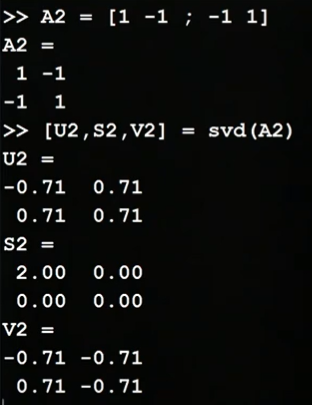
\includegraphics[scale = 0.5]{./figures/SVDex}
\end{figure}

Note that:
\begin{itemize}
        \item the matrix $A_2$ has a rank of 1 as $S_2$ only has 1 non zero value on the diagonal
        \item the absence of a value in the second column of $S_2$ denotes that the second column of $V_2$ is the nullspace of $A_2$
        \item the presence of a value in the first column of $S_2$ denotes to use that the first column of $U_2$ is a basis vector
                for the column space of $A_2$.
\end{itemize}
These analysis are general and so if the above conditions apply, the corresponding inference holds (for SVD)
\pagebreak


\section*{c Matrix Spaces and the SVD}
Consider the following computation:
\begin{figure}[h]
        \centering
        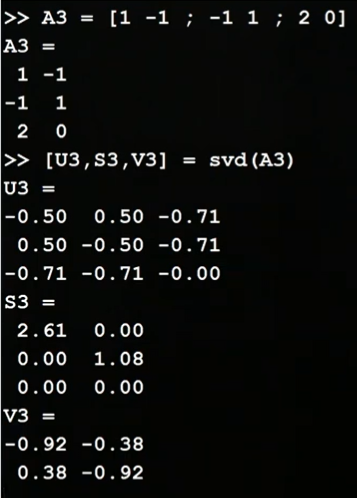
\includegraphics[scale = 0.4]{./figures/MatSVD}
\end{figure}

Note that:
\begin{itemize}
        \item the third vector in $U_3$ is a basis for the complement of the column space of $A_3$
\end{itemize}

Consider the Rank deficient matrix and its computation:
\begin{figure}[h]
        \centering
        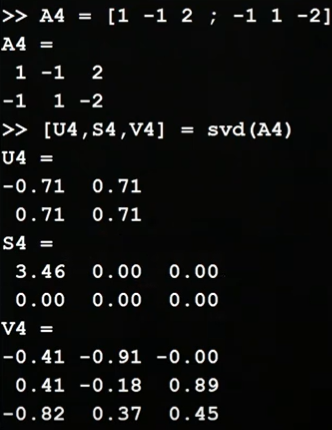
\includegraphics[scale = 0.45]{./figures/MatSVD2}
\end{figure}

Note that:
\begin{itemize}
        \item there is only one non zero value in $S_4$ which means that the rank of $A_4$ is 1
        \item there is a value in the first column of $S_4$
                which means that the first column of $U_4$ is a basis vector for $A_4$
        \item there is no value in column 2 of $S_4$, which means column 2 of $U_4$ is a basis for the complement of the column space of $A$
        \item columns where a 0 value is on the diagonal of $S$ indicates that the corresponding column in $V$ is a basis 
                vector for the nullspace of $A$. Additionally, if a column in  $S$ does not correspond to a column in $A$, then said
                column in $S$ is a basis vector for the nullspace of  $A$
                
                
\end{itemize}




\section*{d Nullspace and the SVD}
Consider a rank deficient matrix: $A\in\mathbb{R}^{m\times m}$
\begin{align*}
        A&\in\mathbb{R}^{2\times 2}\\
        A &= U\Sigma V^\top \\
        U &= \begin{bmatrix} \vec u_1 & \vec u_2 \end{bmatrix}  \\
        \Sigma &= \begin{bmatrix} \sigma_1 & 0 \\ 0 & 0 \end{bmatrix}  \\ 
        V &= \begin{bmatrix} \vec v_1 & \vec v_2 \end{bmatrix}\\
        \vec w &\in \mathbb{R}
.\end{align*}

What is $A\vec w$?
It is the following:
 \[
A\vec w = U\Sigma V^\top\vec w
.\] 
So then what is $V^\top\vec w$
 \[
V^\top\vec w = \begin{bmatrix} \vec v_1^\top \cdot \vec w\\ \vec v_2^\top\cdot \vec w \end{bmatrix} 
.\] 
Note: `$\cdot$' is the dot product.

And continuing to derive the equation:
 \begin{align*}
         \Sigma V^\top\vec w &= \begin{bmatrix} \sigma_1 & 0\\0&0\end{bmatrix}
         \begin{bmatrix} \vec v_1^\top \cdot \vec w\\ \vec v_2^\top\cdot \vec w \end{bmatrix}  \\
        &= \begin{bmatrix} \sigma_1 \vec v_1\cdot \vec w\\ 0 \end{bmatrix}  \\
.\end{align*}
When is the first entry $\sigma_1 \vec v_1\cdot \vec w$ equal to 0?

If and only if $\vec v_1 \cdot \vec w = 0$, which is true when $\vec w\propto \vec v_2 $
Thus, $A\vec w = 0$ if and only if  $\vec w \propto \vec v_2$. 
Therefore the nullspace of $A$ is  $\vec v_2$

\section*{e Orthonormal Basis Vectors and the SVD}
Consider the following computation:
\begin{figure}[h]
        \centering
        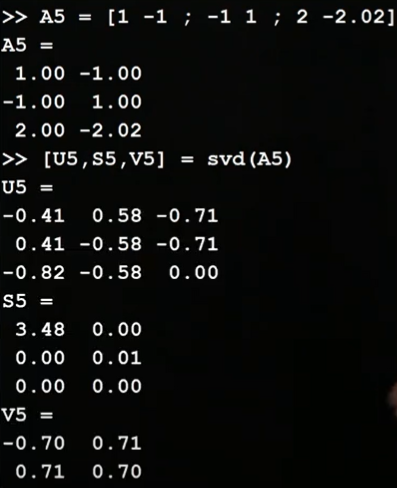
\includegraphics[scale = 0.5]{./figures/Ortho1}
\end{figure}
Note that:
\begin{itemize}
        \item a large ratio between non zero values in $S_5$ is indicative of that the matrix $A_5$ is \textit{almost} rank deficient.
                \[\frac{S_5(1,1)}{S_5(2,2)} = 427.1043\]
                which suggest that an error of 1\% could have a whole number change of 4 on the result.
                If we ignore smaller values like 0.01 we can say that mathematically, this matrix is rank deficient
        \item corresponding vectors in $U_5$ to these smaller values in $S_5$ are `almost' the null space of $A_5$
\end{itemize}

\section*{SVD Properties}
for a general matrix $A\in \mathbb{R}^{m\times n}$
\begin{itemize}
        \item $U\in\mathbb{R}^{m\times m}$ is an Orthonormal basis for the data space of $A$ 
        \item $V\in \mathbb{R}^{n\times n}$ is an Orthonormal basis for the weight space of $A$
        \item  $\Sigma\in\mathbb{R}^{m\times n}$: singular value `diagonal' matrix which is 
                made up of the singular values (pseudo-Eigenvalues)
                of $A$. Same dimensions as  $A$
        \item the last ($n-r$) columns of  $V$ are a basis for the nullspace of  $A$
\end{itemize}

\section*{Learning Summary}
Students should now be able to
\begin{itemize}
        \item  determine the rank of $A$ from SVD
        \item find column space from left singular vectors
        \item find the nullspace from right singular vectors
        \item find the orthogonal complements from  $U$ and  $V$
\end{itemize}
\end{document}

